%%%%%%%%%%%%%%%%%%%%%%%%%%%%%%%%%%%%%%%%%%%%%%%%%%%%%%%%%%%%%%%%%%%%%%
% Lớp 9 | Chương V. Đường tròn | Cung và dây của một đường tròn
% Dạng 9H5?14-3: Liên hệ giữa dây và khoảng cách đến tâm
%%%%%%%%%%%%%%%%%%%%%%%%%%%%%%%%%%%%%%%%%%%%%%%%%%%%%%%%%%%%%%%%%%%%%%


% nguồn: dan_tu_AI (nhập 14/11/2026)
\begin{ex}%[9H5H14-3]%[ma:03f42b79]
	Cho đường tròn $(O;13\text{ cm})$ và dây $AB=24\text{ cm}$. Khoảng cách từ tâm $O$ đến dây $AB$ là
	\choice
	{$12\text{ cm}$}
	{$11\text{ cm}$}
	{\True $5\text{ cm}$}
	{$\sqrt{313}\text{ cm}$}
	\loigiai{
		Kẻ $OH\perp AB$ tại $H$. Tam giác $OAB$ cân tại $O$ nên $H$ là trung điểm $AB$, $HA=12\text{ cm}$.\\
		$OH=\sqrt{OA^2-HA^2}=\sqrt{169-144}=5\text{ (cm)}$.
	}
\end{ex}

% nguồn: dan_tu_AI (nhập 14/11/2026)
\begin{ex}%[9H5H14-3]%[ma:8dbf635e]
	Cho đường tròn $(O;10\text{ cm})$ và hai dây $AB=16\text{ cm}$, $CD=12\text{ cm}$. Các khẳng định sau đúng hay sai?
	\choiceTF
	{\True Khoảng cách từ $O$ đến dây $AB$ bằng $6\text{ cm}$}
	{\True Khoảng cách từ $O$ đến dây $CD$ bằng $8\text{ cm}$}
	{Dây $CD$ gần tâm $O$ hơn dây $AB$}
	{Nếu $AB\parallel CD$ và tâm $O$ nằm giữa hai dây thì khoảng cách giữa hai dây bằng $2\text{ cm}$}
	\loigiai{
		\begin{itemchoice}
			\itemch Đúng. Kẻ $OH\perp AB$ thì $H$ là trung điểm $AB$, $OH=\sqrt{10^2-8^2}=6\text{ (cm)}$.
			\itemch Đúng. Kẻ $OK\perp CD$ thì $K$ là trung điểm $CD$, $OK=\sqrt{10^2-6^2}=8\text{ (cm)}$.
			\itemch Sai. $OH=6<8=OK$ nên dây $AB$ gần tâm hơn dây $CD$.
			\itemch Sai. Khi $O$ nằm giữa hai dây song song thì $H$, $O$, $K$ thẳng hàng và khoảng cách giữa hai dây là $HK=OH+OK=6+8=14\text{ (cm)}$.
		\end{itemchoice}
	}
\end{ex}

% nguồn: dan_tu_AI (nhập 14/11/2026)
\begin{bt}%[9H5C14-3]%[ma:1c204464]
	Cho đường tròn $(O;R)$ có hai dây song song $AB=24\text{ cm}$ và $CD=10\text{ cm}$, tâm $O$ nằm giữa hai dây. Khoảng cách giữa hai dây là $17\text{ cm}$. Tính bán kính $R$ (đơn vị: cm).
	\shortans{13}
	\loigiai{
		Kẻ đường thẳng qua $O$ vuông góc với hai dây, cắt $AB$, $CD$ tại $H$, $K$. Khi đó $H$, $K$ là trung điểm của $AB$, $CD$ và $OH+OK=HK=17$.\\
		Đặt $OH=x$, $OK=17-x$ ($0<x<17$). Ta có
		\[ R^2=x^2+12^2=(17-x)^2+5^2. \]
		$\Leftrightarrow x^2+144=289-34x+x^2+25\Leftrightarrow 34x=170\Leftrightarrow x=5$.\\
		Vậy $R=\sqrt{5^2+12^2}=13\text{ (cm)}$.
	}
\end{bt}

% nguồn: dan_tu_AI (nhập 18/11/2026)
\begin{bt}%[9H5H14-3]%[ma:21958253]
	Cho đường tròn $(O; 13\text{ cm})$. Trong đường tròn vẽ hai dây $AB = 24\text{ cm}$ và $CD = 10\text{ cm}$. 
	\begin{enumerate}
		\item Tính khoảng cách từ tâm $O$ đến dây $AB$ và dây $CD$.
		\item Dây nào gần tâm hơn? Vì sao?
	\end{enumerate}
	\loigiai{
		\begin{center}
			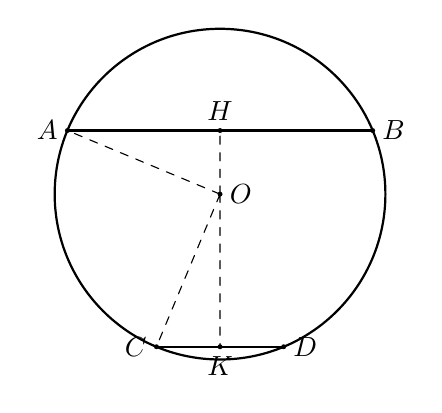
\begin{tikzpicture}[scale=0.6,>=stealth, line join=round, line cap=round]
				\def\R{3.5}
				\coordinate (O) at (0,0);
				\draw[thick] (O) circle (\R);
				% AB length 24 ~ radius 13 -> half is 12. dist = 5.
				\coordinate (H) at (0, 1.346); % 5/13 * 3.5
				\coordinate (A) at (-3.23, 1.346); % 12/13 * 3.5
				\coordinate (B) at (3.23, 1.346);
				% CD length 10 -> half is 5. dist = 12.
				\coordinate (K) at (0, -3.23); % 12/13 * 3.5
				\coordinate (C) at (-1.346, -3.23); % 5/13 * 3.5
				\coordinate (D) at (1.346, -3.23);
				\draw[thick] (A)--(B) node[midway, above] {};
				\draw[thick] (C)--(D) node[midway, below] {};
				\draw[dashed] (O)--(A) (O)--(C) (O)--(H) (O)--(K);
				\fill (O) circle (1.5pt) node[right] {$O$};
				\fill (A) circle (1.5pt) node[left] {$A$};
				\fill (B) circle (1.5pt) node[right] {$B$};
				\fill (C) circle (1.5pt) node[left] {$C$};
				\fill (D) circle (1.5pt) node[right] {$D$};
				\fill (H) circle (1.5pt) node[above] {$H$};
				\fill (K) circle (1.5pt) node[below] {$K$};
				\tkzMarkRightAngle[size=0.2](O,H,A);
				\tkzMarkRightAngle[size=0.2](O,K,C);
			\end{tikzpicture}
		\end{center}
		\begin{enumerate}
			\item Kẻ $OH \perp AB$ tại $H$ và $OK \perp CD$ tại $K$.\\
			Vì $OH \perp AB$ nên $H$ là trung điểm của $AB$ (định lí đường kính vuông góc với dây).\\
			Suy ra $AH = \dfrac{AB}{2} = \dfrac{24}{2} = 12\text{ (cm)}$.\\
			Xét tam giác vuông $OHA$, theo định lí Pythagore ta có:\\
			$OH = \sqrt{OA^2 - AH^2} = \sqrt{13^2 - 12^2} = \sqrt{169 - 144} = \sqrt{25} = 5\text{ (cm)}$.\\
			Tương tự, vì $OK \perp CD$ nên $K$ là trung điểm của $CD$.\\
			Suy ra $CK = \dfrac{CD}{2} = \dfrac{10}{2} = 5\text{ (cm)}$.\\
			Xét tam giác vuông $OKC$, theo định lí Pythagore ta có:\\
			$OK = \sqrt{OC^2 - CK^2} = \sqrt{13^2 - 5^2} = \sqrt{169 - 25} = \sqrt{144} = 12\text{ (cm)}$.\\
			Vậy khoảng cách từ $O$ đến $AB$ là $5\text{ cm}$, từ $O$ đến $CD$ là $12\text{ cm}$.
			\item Ta có khoảng cách từ tâm $O$ đến $AB$ là $OH = 5\text{ cm}$, khoảng cách từ tâm $O$ đến $CD$ là $OK = 12\text{ cm}$.\\
			Vì $5 < 12$ nên $OH < OK$. Do đó, dây $AB$ gần tâm hơn dây $CD$.\\
			\textit{(Lưu ý: Học sinh cũng có thể giải thích dựa vào độ dài dây: vì $AB = 24\text{ cm} > CD = 10\text{ cm}$ nên dây $AB$ lớn hơn sẽ gần tâm hơn).}
		\end{enumerate}
	}
\end{bt}

% nguồn: dan_tu_AI (nhập 18/11/2026)
\begin{bt}%[9H5H14-3]%[ma:851e8f38]
	Cho đường tròn $(O)$ có hai dây $AB$ và $CD$ bằng nhau và cắt nhau tại điểm $M$ nằm trong đường tròn. Gọi $H$ và $K$ lần lượt là hình chiếu vuông góc của $O$ trên dây $AB$ và dây $CD$. Chứng minh rằng $MH = MK$.
	\loigiai{
		\begin{center}
			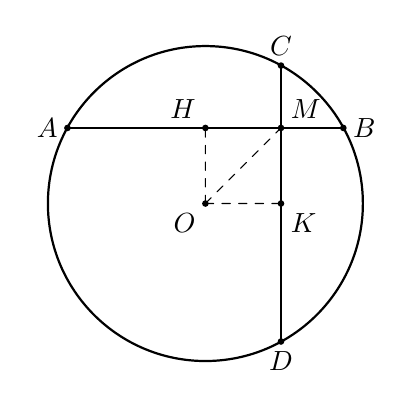
\begin{tikzpicture}[scale=0.8,>=stealth, line join=round, line cap=round]
				\def\R{2.5}
				\coordinate (O) at (0,0);
				\draw[thick] (O) circle (\R);
				\coordinate (H) at (0, 1.2);
				\coordinate (A) at (-2.19, 1.2); % sqrt(2.5^2 - 1.2^2) = 2.19
				\coordinate (B) at (2.19, 1.2);
				\coordinate (K) at (1.2, 0);
				\coordinate (C) at (1.2, 2.19);
				\coordinate (D) at (1.2, -2.19);
				\draw[thick] (A)--(B);
				\draw[thick] (C)--(D);
				\coordinate (M) at (1.2, 1.2);
				\draw[dashed] (O)--(H) (O)--(K) (O)--(M);
				\fill (O) circle (1.5pt) node[below left] {$O$};
				\fill (M) circle (1.5pt) node[above right] {$M$};
				\fill (H) circle (1.5pt) node[above left] {$H$};
				\fill (K) circle (1.5pt) node[below right] {$K$};
				\fill (A) circle (1.5pt) node[left] {$A$};
				\fill (B) circle (1.5pt) node[right] {$B$};
				\fill (C) circle (1.5pt) node[above] {$C$};
				\fill (D) circle (1.5pt) node[below] {$D$};
				\tkzMarkRightAngle[size=0.2](O,H,A);
				\tkzMarkRightAngle[size=0.2](O,K,D);
			\end{tikzpicture}
		\end{center}
		Vì $H$ và $K$ lần lượt là hình chiếu của $O$ trên $AB$ và $CD$ nên $OH \perp AB$ và $OK \perp CD$.\\
		Khoảng cách từ tâm $O$ đến dây $AB$ là $OH$, khoảng cách từ $O$ đến dây $CD$ là $OK$.\\
		Theo giả thiết, hai dây bằng nhau ($AB = CD$) nên chúng cách đều tâm, suy ra $OH = OK$.\\
		Xét hai tam giác vuông $\Delta OHM$ (vuông tại $H$) và $\Delta OKM$ (vuông tại $K$) có:\\
		Cạnh huyền $OM$ chung;\\
		Cạnh góc vuông $OH = OK$ (chứng minh trên).\\
		Do đó $\Delta OHM = \Delta OKM$ (cạnh huyền - cạnh góc vuông).\\
		Suy ra $MH = MK$ (hai cạnh tương ứng).
	}
\end{bt}

% nguồn: 2026-11-21_lop9_chuong5_bai14_17 (nhập 21/11/2026)
\begin{ex}%[9H5N14-3]%[ma:0972c56e]
% nguon: SGK Toán 9 KNTT tập 1 – Bài 14, Cung và dây của một đường tròn
	Cho đường tròn $(O; 13\text{ cm})$ và dây $AB = 24\text{ cm}$. Khoảng cách từ tâm $O$ đến dây $AB$ bằng
	\choice
	{\True $5\text{ cm}$}
	{$6\text{ cm}$}
	{$11\text{ cm}$}
	{$12\text{ cm}$}
	\loigiai{
		Gọi $H$ là trung điểm của dây $AB$, ta có $OH \perp AB$ và $AH = \dfrac{AB}{2} = 12\text{ cm}$.\\
		Trong tam giác $OHA$ vuông tại $H$: $OH = \sqrt{OA^2 - AH^2} = \sqrt{13^2 - 12^2} = 5\text{ cm}$.
	}
\end{ex}

% nguồn: 2026-11-21_lop9_chuong5_bai14_17 (nhập 21/11/2026)
\begin{ex}%[9H5H14-3]%[ma:bb5c73dd]
% nguon: SGK Toán 9 KNTT tập 1 – Bài 14, Cung và dây của một đường tròn
	Cho đường tròn $(O; 10\text{ cm})$ có hai dây song song $AB = 12\text{ cm}$ và $CD = 16\text{ cm}$ nằm cùng một phía đối với tâm $O$. Xét tính đúng, sai của các khẳng định sau:
	\choiceTF
	{\True Khoảng cách từ tâm $O$ đến dây $AB$ bằng $8\text{ cm}$}
	{\True Khoảng cách từ tâm $O$ đến dây $CD$ bằng $6\text{ cm}$}
	{Khoảng cách giữa hai dây song song $AB$ và $CD$ bằng $14\text{ cm}$}
	{\True Diện tích hình thang $ABCD$ bằng $28\text{ cm}^2$}
	\loigiai{
		\begin{itemchoice}
			\itemch Đúng. Gọi $H$ là trung điểm $AB$, ta có $AH = 6\text{ cm}$ nên $OH = \sqrt{10^2 - 6^2} = 8\text{ cm}$.
			\itemch Đúng. Gọi $K$ là trung điểm $CD$, ta có $CK = 8\text{ cm}$ nên $OK = \sqrt{10^2 - 8^2} = 6\text{ cm}$.
			\itemch Sai. Vì hai dây $AB$ và $CD$ nằm cùng một phía đối với tâm $O$ nên khoảng cách giữa chúng là $HK = OH - OK = 8 - 6 = 2\text{ cm}$.
			\itemch Đúng. Hình thang $ABCD$ có hai đáy $AB = 12\text{ cm}$, $CD = 16\text{ cm}$ và chiều cao $HK = 2\text{ cm}$ nên diện tích là $\dfrac{12 + 16}{2} \cdot 2 = 28\text{ cm}^2$.
		\end{itemchoice}
	}
\end{ex}

% nguồn: 2026-11-21_lop9_chuong5_bai14_17 (nhập 21/11/2026)
\begin{bt}%[9H5V14-3]%[ma:b48da136]
% nguon: SGK Toán 9 KNTT tập 1 – Bài 14, Cung và dây của một đường tròn
	Một đường ống nước hình trụ nằm ngang có mặt cắt ngang là hình tròn bán kính $25\text{ cm}$. Khi mực nước trong ống sâu $10\text{ cm}$ (tính từ điểm thấp nhất của đáy ống lên mặt nước) thì bề rộng mặt thoáng của nước trong ống bằng bao nhiêu xăng-ti-mét?
	\shortans{40}
	\loigiai{
		Gọi $O$ là tâm mặt cắt tròn bán kính $R = 25\text{ cm}$, $AB$ là dây biểu thị mặt thoáng của nước.\\
		Khoảng cách từ tâm $O$ đến mặt thoáng $AB$ là $d = 25 - 10 = 15\text{ cm}$.\\
		Nửa bề rộng mặt thoáng là $\sqrt{25^2 - 15^2} = \sqrt{400} = 20\text{ cm}$.\\
		Vậy bề rộng mặt thoáng của nước là $AB = 2 \cdot 20 = 40\text{ cm}$.
	}
\end{bt}

% nguồn: 2026-11-21_lop9_chuong5_bai14_15_bs (nhập 21/11/2026)
\begin{ex}%[9H5N14-3]%[ma:6cafc43d]
% nguon: SGK Toán 9 KNTT tập 1 – Bài 14, Cung và dây của một đường tròn
	Trong một đường tròn, hai dây bằng nhau khi và chỉ khi
	\choice
	{\True Hai dây đó cách đều tâm}
	{Hai dây đó song song với nhau}
	{Hai dây đó vuông góc với nhau}
	{Hai dây đó cắt nhau tại tâm}
	\loigiai{
		Theo tính chất liên hệ giữa dây và khoảng cách từ tâm đến dây, trong một đường tròn, hai dây bằng nhau khi và chỉ khi chúng cách đều tâm.
	}
\end{ex}

% nguồn: 2026-11-21_lop9_chuong5_bai14_15_bs (nhập 21/11/2026)
\begin{ex}%[9H5N14-3]%[ma:bd31a985]
% nguon: SGK Toán 9 KNTT tập 1 – Bài 14, Cung và dây của một đường tròn
	Cho đường tròn $(O; 10\text{ cm})$ và dây $CD = 12\text{ cm}$. Khoảng cách từ tâm $O$ đến dây $CD$ bằng
	\choice
	{$4\text{ cm}$}
	{$6\text{ cm}$}
	{\True $8\text{ cm}$}
	{$9\text{ cm}$}
	\loigiai{
		Gọi $K$ là trung điểm dây $CD$, ta có $OK \perp CD$ và $CK = 6\text{ cm}$.\\
		Trong tam giác $OKC$ vuông tại $K$: $OK = \sqrt{10^2 - 6^2} = 8\text{ cm}$.
	}
\end{ex}

% nguồn: 2026-11-21_lop9_chuong5_bai14_15_bs (nhập 21/11/2026)
\begin{ex}%[9H5H14-3]%[ma:f291e492]
% nguon: SGK Toán 9 KNTT tập 1 – Bài 14, Cung và dây của một đường tròn
	Cho đường tròn $(O; 13\text{ cm})$ có hai dây $AB = 10\text{ cm}$ và $CD = 24\text{ cm}$. Xét tính đúng, sai của các khẳng định sau:
	\choiceTF
	{\True Khoảng cách từ tâm $O$ đến dây $AB$ bằng $12\text{ cm}$}
	{\True Khoảng cách từ tâm $O$ đến dây $CD$ bằng $5\text{ cm}$}
	{Dây $AB$ gần tâm $O$ hơn dây $CD$}
	{\True Nếu $AB \parallel CD$ và hai dây nằm khác phía đối với tâm $O$ thì khoảng cách giữa hai dây bằng $17\text{ cm}$}
	\loigiai{
		\begin{itemchoice}
			\itemch Đúng. Khoảng cách từ $O$ đến $AB$ là $\sqrt{13^2 - 5^2} = 12\text{ cm}$.
			\itemch Đúng. Khoảng cách từ $O$ đến $CD$ là $\sqrt{13^2 - 12^2} = 5\text{ cm}$.
			\itemch Sai. Vì $5 < 12$ nên dây $CD$ gần tâm $O$ hơn dây $AB$ (dây lớn hơn thì gần tâm hơn).
			\itemch Đúng. Khi hai dây song song nằm khác phía đối với tâm $O$, khoảng cách giữa chúng bằng tổng hai khoảng cách từ tâm đến mỗi dây: $12 + 5 = 17\text{ cm}$.
		\end{itemchoice}
	}
\end{ex}

% nguồn: 2026-11-21_lop9_chuong5_bai14_15_bs (nhập 21/11/2026)
\begin{ex}%[9H5H14-3]%[ma:513329d8]
% nguon: SGK Toán 9 KNTT tập 1 – Bài 14, Cung và dây của một đường tròn
	Cho đường tròn $(O; 5\text{ cm})$ và điểm $M$ nằm trong đường tròn sao cho $OM = 3\text{ cm}$. Xét các dây của đường tròn đi qua điểm $M$:
	\choiceTF
	{\True Dây lớn nhất đi qua $M$ có độ dài bằng $10\text{ cm}$}
	{\True Dây ngắn nhất đi qua $M$ vuông góc với $OM$ tại $M$}
	{Độ dài dây ngắn nhất đi qua $M$ bằng $6\text{ cm}$}
	{\True Diện tích tam giác tạo bởi tâm $O$ và hai đầu mút của dây ngắn nhất đi qua $M$ bằng $12\text{ cm}^2$}
	\loigiai{
		\begin{itemchoice}
			\itemch Đúng. Dây lớn nhất đi qua $M$ là đường kính đi qua $M$, có độ dài $2R = 10\text{ cm}$.
			\itemch Đúng. Khoảng cách từ $O$ đến mọi dây đi qua $M$ đều không vượt quá $OM$, đạt lớn nhất bằng $OM$ khi dây vuông góc với $OM$ tại $M$, khi đó dây có độ dài nhỏ nhất.
			\itemch Sai. Độ dài dây ngắn nhất là $2\sqrt{5^2 - 3^2} = 2 \cdot 4 = 8\text{ cm}$.
			\itemch Đúng. Diện tích tam giác tạo bởi $O$ và dây ngắn nhất là $\dfrac{1}{2} \cdot 8 \cdot 3 = 12\text{ cm}^2$.
		\end{itemchoice}
	}
\end{ex}

% nguồn: 2026-11-21_lop9_chuong5_bai14_15_bs (nhập 21/11/2026)
\begin{bt}%[9H5V14-3]%[ma:ab1d56c3]
% nguon: SGK Toán 9 KNTT tập 1 – Bài 14, Cung và dây của một đường tròn
	Cho đường tròn $(O; 17\text{ cm})$ có hai dây song song $AB = 16\text{ cm}$ và $CD = 30\text{ cm}$ nằm về hai phía đối với tâm $O$. Tính khoảng cách giữa hai dây $AB$ và $CD$ (đơn vị cm).
	\shortans{23}
	\loigiai{
		Khoảng cách từ tâm $O$ đến dây $AB$ là $d_1 = \sqrt{17^2 - 8^2} = \sqrt{225} = 15\text{ cm}$.\\
		Khoảng cách từ tâm $O$ đến dây $CD$ là $d_2 = \sqrt{17^2 - 15^2} = \sqrt{64} = 8\text{ cm}$.\\
		Vì hai dây song song nằm về hai phía của tâm $O$ nên khoảng cách giữa chúng là $d_1 + d_2 = 15 + 8 = 23\text{ cm}$.
	}
\end{bt}

% nguồn: 2026-11-21_lop9_chuong5_bai14_15_bs (nhập 21/11/2026)
\begin{bt}%[9H5V14-3]%[ma:7b226585]
% nguon: SGK Toán 9 KNTT tập 1 – Bài 14, Cung và dây của một đường tròn
	Một cổng vòm có dạng cung tròn bán kính $5\text{ m}$, bề rộng chân vòm (dây cung trên mặt đất) là $8\text{ m}$ và tâm đường tròn nằm dưới mặt đất. Tính chiều cao lớn nhất của cổng vòm tính từ mặt đất đến đỉnh vòm (đơn vị mét).
	\shortans{2}
	\loigiai{
		Khoảng cách từ tâm đường tròn đến dây cung mặt đất là $d = \sqrt{5^2 - 4^2} = 3\text{ m}$.\\
		Chiều cao lớn nhất từ mặt đất đến đỉnh vòm bằng $R - d = 5 - 3 = 2\text{ m}$.
	}
\end{bt}
